% Options for packages loaded elsewhere
\PassOptionsToPackage{unicode}{hyperref}
\PassOptionsToPackage{hyphens}{url}
\PassOptionsToPackage{dvipsnames,svgnames,x11names}{xcolor}
%
\documentclass[
  letterpaper,
  DIV=11,
  numbers=noendperiod]{scrartcl}

\usepackage{amsmath,amssymb}
\usepackage{iftex}
\ifPDFTeX
  \usepackage[T1]{fontenc}
  \usepackage[utf8]{inputenc}
  \usepackage{textcomp} % provide euro and other symbols
\else % if luatex or xetex
  \usepackage{unicode-math}
  \defaultfontfeatures{Scale=MatchLowercase}
  \defaultfontfeatures[\rmfamily]{Ligatures=TeX,Scale=1}
\fi
\usepackage{lmodern}
\ifPDFTeX\else  
    % xetex/luatex font selection
\fi
% Use upquote if available, for straight quotes in verbatim environments
\IfFileExists{upquote.sty}{\usepackage{upquote}}{}
\IfFileExists{microtype.sty}{% use microtype if available
  \usepackage[]{microtype}
  \UseMicrotypeSet[protrusion]{basicmath} % disable protrusion for tt fonts
}{}
\makeatletter
\@ifundefined{KOMAClassName}{% if non-KOMA class
  \IfFileExists{parskip.sty}{%
    \usepackage{parskip}
  }{% else
    \setlength{\parindent}{0pt}
    \setlength{\parskip}{6pt plus 2pt minus 1pt}}
}{% if KOMA class
  \KOMAoptions{parskip=half}}
\makeatother
\usepackage{xcolor}
\setlength{\emergencystretch}{3em} % prevent overfull lines
\setcounter{secnumdepth}{-\maxdimen} % remove section numbering
% Make \paragraph and \subparagraph free-standing
\ifx\paragraph\undefined\else
  \let\oldparagraph\paragraph
  \renewcommand{\paragraph}[1]{\oldparagraph{#1}\mbox{}}
\fi
\ifx\subparagraph\undefined\else
  \let\oldsubparagraph\subparagraph
  \renewcommand{\subparagraph}[1]{\oldsubparagraph{#1}\mbox{}}
\fi


\providecommand{\tightlist}{%
  \setlength{\itemsep}{0pt}\setlength{\parskip}{0pt}}\usepackage{longtable,booktabs,array}
\usepackage{calc} % for calculating minipage widths
% Correct order of tables after \paragraph or \subparagraph
\usepackage{etoolbox}
\makeatletter
\patchcmd\longtable{\par}{\if@noskipsec\mbox{}\fi\par}{}{}
\makeatother
% Allow footnotes in longtable head/foot
\IfFileExists{footnotehyper.sty}{\usepackage{footnotehyper}}{\usepackage{footnote}}
\makesavenoteenv{longtable}
\usepackage{graphicx}
\makeatletter
\def\maxwidth{\ifdim\Gin@nat@width>\linewidth\linewidth\else\Gin@nat@width\fi}
\def\maxheight{\ifdim\Gin@nat@height>\textheight\textheight\else\Gin@nat@height\fi}
\makeatother
% Scale images if necessary, so that they will not overflow the page
% margins by default, and it is still possible to overwrite the defaults
% using explicit options in \includegraphics[width, height, ...]{}
\setkeys{Gin}{width=\maxwidth,height=\maxheight,keepaspectratio}
% Set default figure placement to htbp
\makeatletter
\def\fps@figure{htbp}
\makeatother

\KOMAoption{captions}{tableheading}
\makeatletter
\makeatother
\makeatletter
\makeatother
\makeatletter
\@ifpackageloaded{caption}{}{\usepackage{caption}}
\AtBeginDocument{%
\ifdefined\contentsname
  \renewcommand*\contentsname{Table of contents}
\else
  \newcommand\contentsname{Table of contents}
\fi
\ifdefined\listfigurename
  \renewcommand*\listfigurename{List of Figures}
\else
  \newcommand\listfigurename{List of Figures}
\fi
\ifdefined\listtablename
  \renewcommand*\listtablename{List of Tables}
\else
  \newcommand\listtablename{List of Tables}
\fi
\ifdefined\figurename
  \renewcommand*\figurename{Figure}
\else
  \newcommand\figurename{Figure}
\fi
\ifdefined\tablename
  \renewcommand*\tablename{Table}
\else
  \newcommand\tablename{Table}
\fi
}
\@ifpackageloaded{float}{}{\usepackage{float}}
\floatstyle{ruled}
\@ifundefined{c@chapter}{\newfloat{codelisting}{h}{lop}}{\newfloat{codelisting}{h}{lop}[chapter]}
\floatname{codelisting}{Listing}
\newcommand*\listoflistings{\listof{codelisting}{List of Listings}}
\makeatother
\makeatletter
\@ifpackageloaded{caption}{}{\usepackage{caption}}
\@ifpackageloaded{subcaption}{}{\usepackage{subcaption}}
\makeatother
\makeatletter
\@ifpackageloaded{tcolorbox}{}{\usepackage[skins,breakable]{tcolorbox}}
\makeatother
\makeatletter
\@ifundefined{shadecolor}{\definecolor{shadecolor}{rgb}{.97, .97, .97}}
\makeatother
\makeatletter
\makeatother
\makeatletter
\makeatother
\ifLuaTeX
  \usepackage{selnolig}  % disable illegal ligatures
\fi
\IfFileExists{bookmark.sty}{\usepackage{bookmark}}{\usepackage{hyperref}}
\IfFileExists{xurl.sty}{\usepackage{xurl}}{} % add URL line breaks if available
\urlstyle{same} % disable monospaced font for URLs
\hypersetup{
  colorlinks=true,
  linkcolor={blue},
  filecolor={Maroon},
  citecolor={Blue},
  urlcolor={Blue},
  pdfcreator={LaTeX via pandoc}}

\author{}
\date{}

\begin{document}
\ifdefined\Shaded\renewenvironment{Shaded}{\begin{tcolorbox}[breakable, interior hidden, borderline west={3pt}{0pt}{shadecolor}, frame hidden, boxrule=0pt, sharp corners, enhanced]}{\end{tcolorbox}}\fi

\hypertarget{basic-data-exploration}{%
\section{\texorpdfstring{\textbf{Basic Data
Exploration}}{Basic Data Exploration}}\label{basic-data-exploration}}

\hypertarget{performing-descriptive-statistics-on-time-series-data}{%
\subsection{Performing descriptive statistics on time series
data}\label{performing-descriptive-statistics-on-time-series-data}}

In the previous chapter, the process of creating a new workfile and
importing data into eviews was demonstrated. Visit chapter one of the
material if you have not done so.

We will open the stockindex workfile we save in the previous chapter.
The workfile contains timeseries data on various stock indixes from
different stock markets.

\hypertarget{open-an-existing-workfile}{%
\subsubsection{Open an Existing
Workfile}\label{open-an-existing-workfile}}

\begin{enumerate}
\def\labelenumi{\arabic{enumi}.}
\item
  Click file -\textgreater{} New -\textgreater Workfile
\item
  Open the stockindex workfile created

  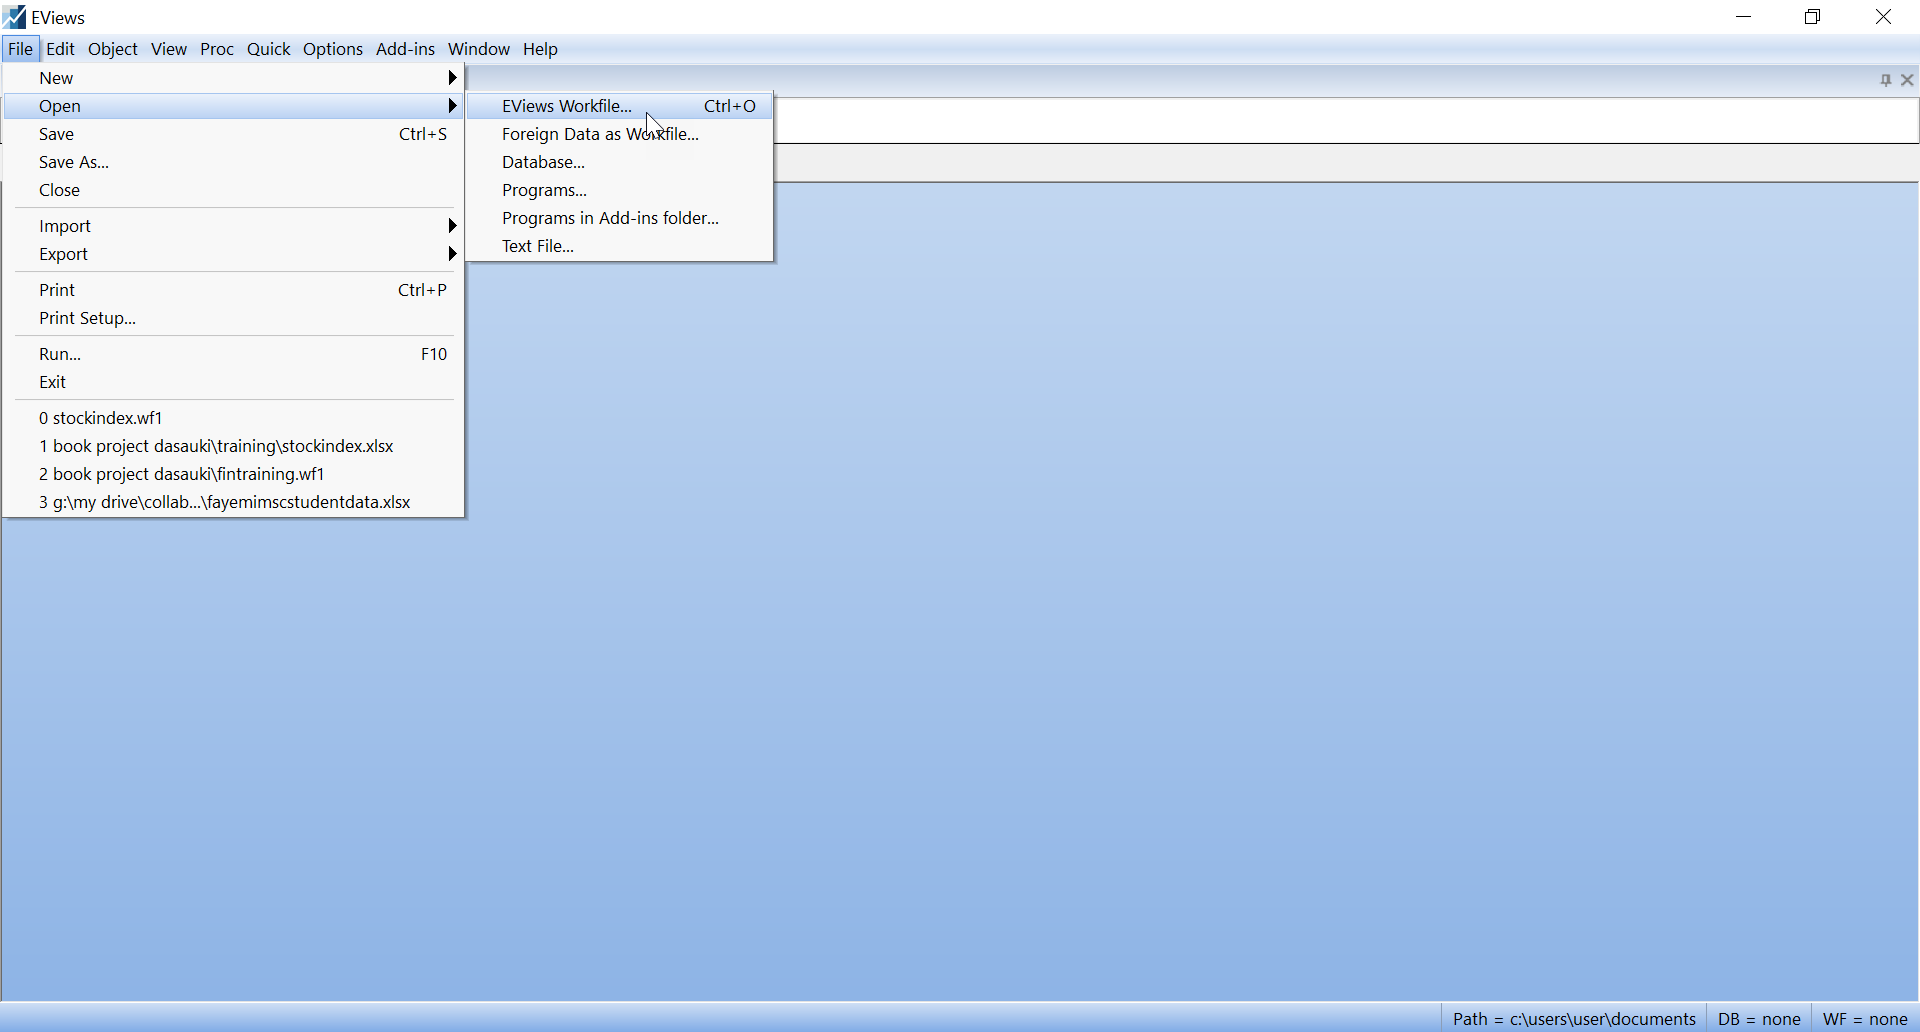
\includegraphics{images/openworkfile.png}
\item
  A pop up window appears as shown below. brow to the location of
  stockindex file
\item
  click on the stockindex file (the name may differ on you computer,
  depending on the name you saved as).

  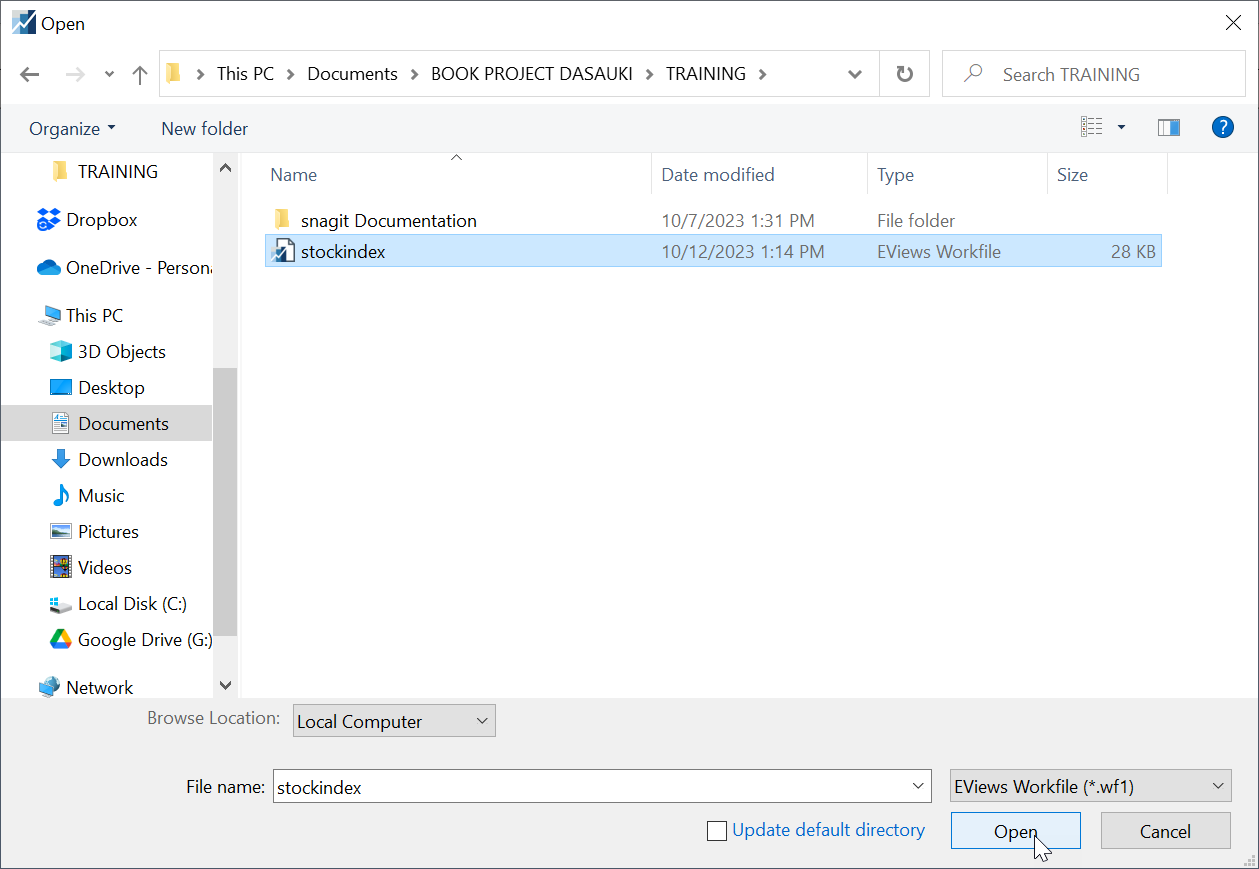
\includegraphics{images/openworkfile2.png}
\item
  click on open to open the work file.

  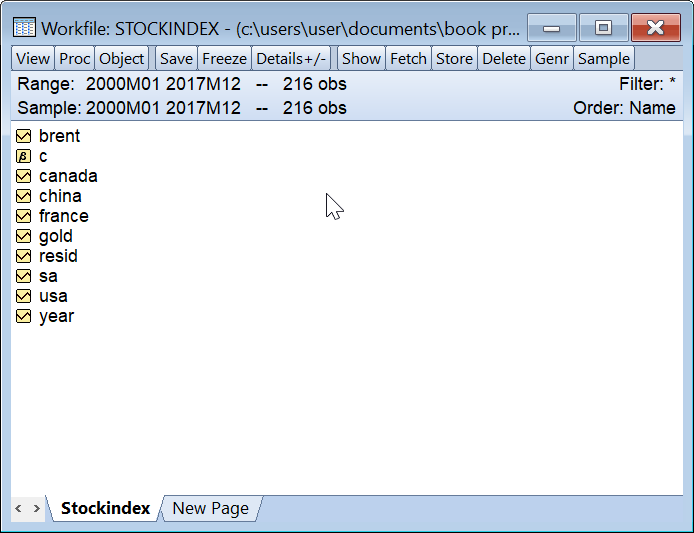
\includegraphics{images/saveworkfile3.png}
\end{enumerate}

now the data file (stockindex) has been imported and we are ready to run
the descriptive statistics. You will notice that the workfile consists
of several objects including brent, canada, usa, gold sa, france, china
as well as resid and c - the constant which were generated automatically
when the work file was created. each object contains the data for the
variable it is named with. for instant the object gold, contains the
data for the variable called gold. This test will compute statistics
such as mean median, mode, standard deviation, kurtosis, skewness and
others.

\hypertarget{step-2-view-your-data}{%
\subsubsection{\texorpdfstring{\textbf{Step 2: View Your
Data}}{Step 2: View Your Data}}\label{step-2-view-your-data}}

the first step is to view any one of the variables you intend to compute
the statistics for.

\begin{enumerate}
\def\labelenumi{\arabic{enumi}.}
\item
  move your mouse cursor to the variable of interest and right click on
  the variable.
\item
  Click on open.

  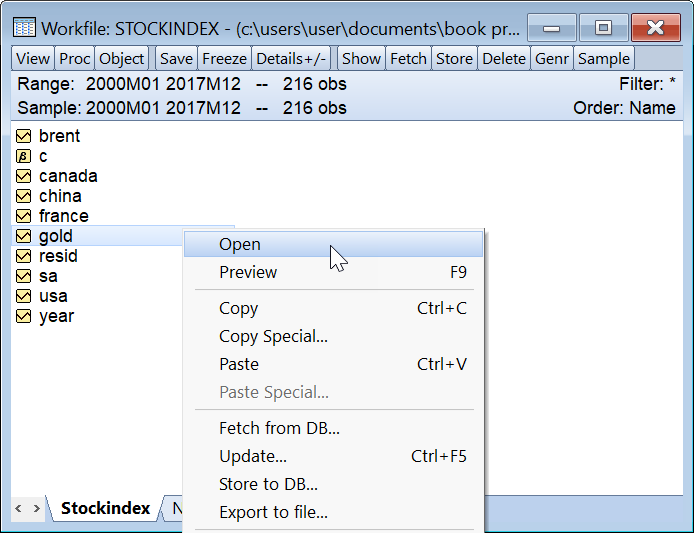
\includegraphics{images/viewdata1.png}

  Alternative, you should simple double click on the variable of
  interest to view the data in the object.
\item
  In the workfile window, you'll see your dataset loaded as a
  spreadsheet. You can scroll through the data to get a sense of its
  structure and content.

  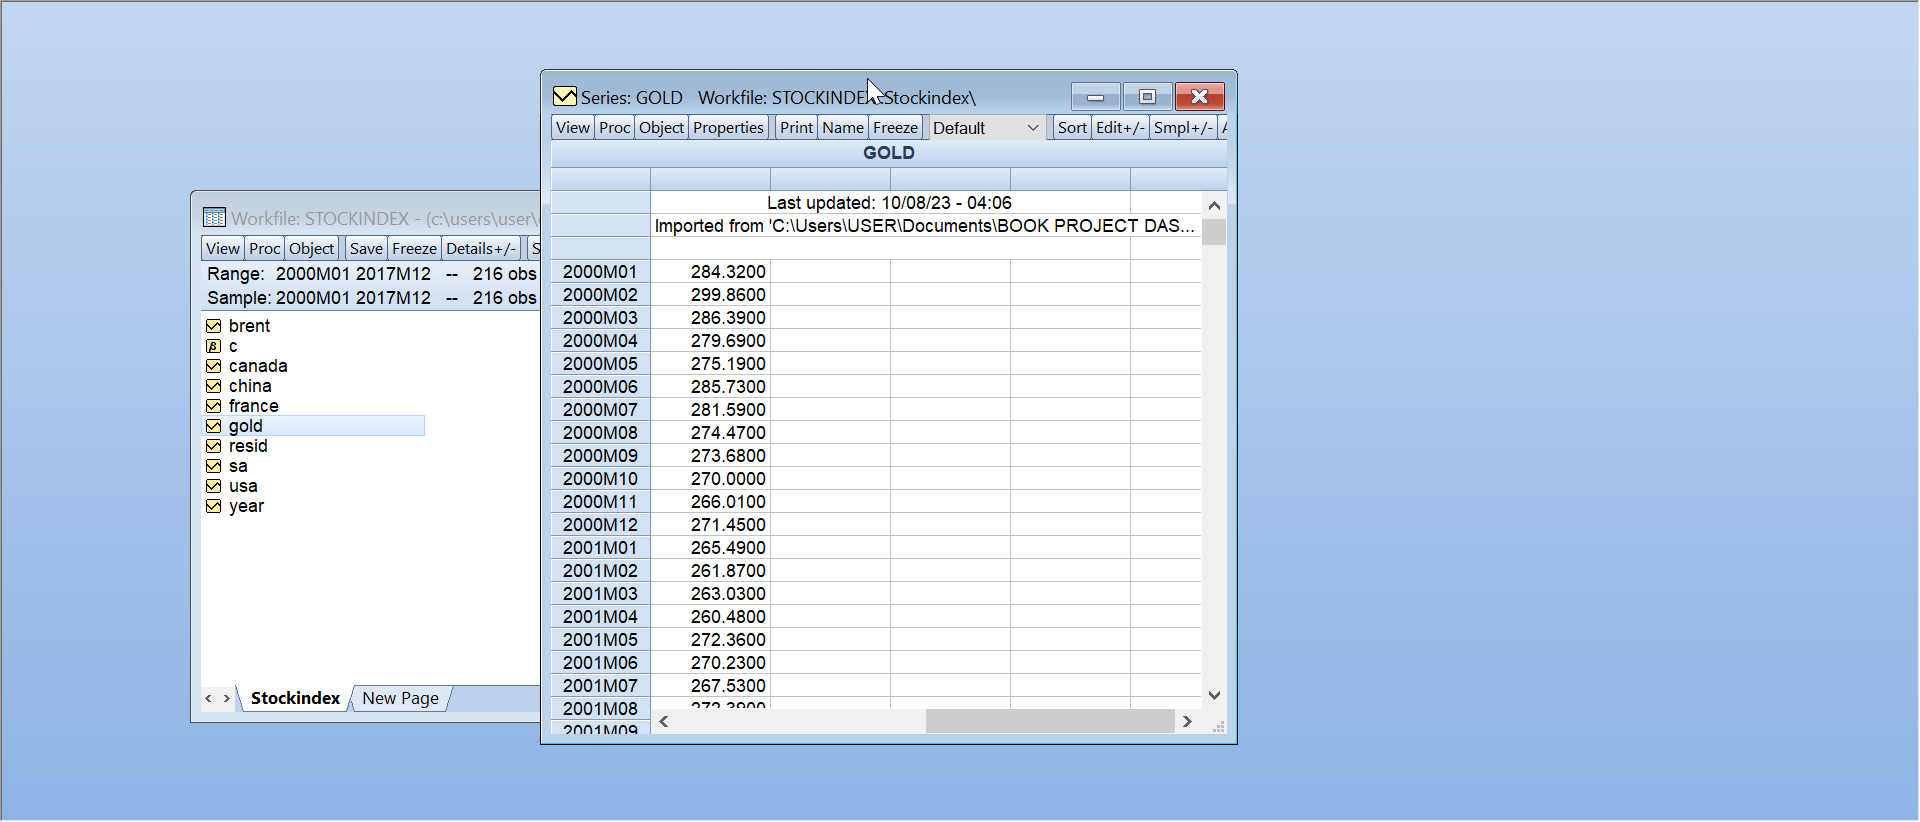
\includegraphics{images/viewdata2.png}
\end{enumerate}

\hypertarget{step-3-descriptive-statistics-for-numeric-variables}{%
\subsubsection{\texorpdfstring{\textbf{Step 3: Descriptive Statistics
for Numeric
Variables}}{Step 3: Descriptive Statistics for Numeric Variables}}\label{step-3-descriptive-statistics-for-numeric-variables}}

From the page displaying the data contained in the object ``gold'', do
the following to implement descriptive statistics:

\begin{enumerate}
\def\labelenumi{\arabic{enumi}.}
\tightlist
\item
  click on view \textgreater{} descriptive statistics \& test
  \textgreater{} Histogram \& stats
\end{enumerate}

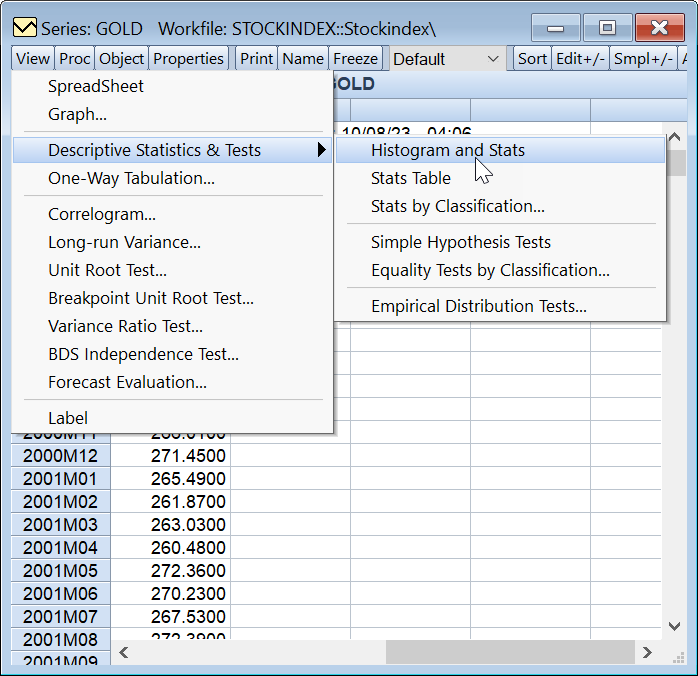
\includegraphics{images/descriptive1.png}

Alternatively:

\begin{enumerate}
\def\labelenumi{\arabic{enumi}.}
\item
  Go to ``View'' \textgreater{} ``Quick'' \textgreater{} ``Descriptive
  Statistics.'' \textgreater Histogram \& Stats

  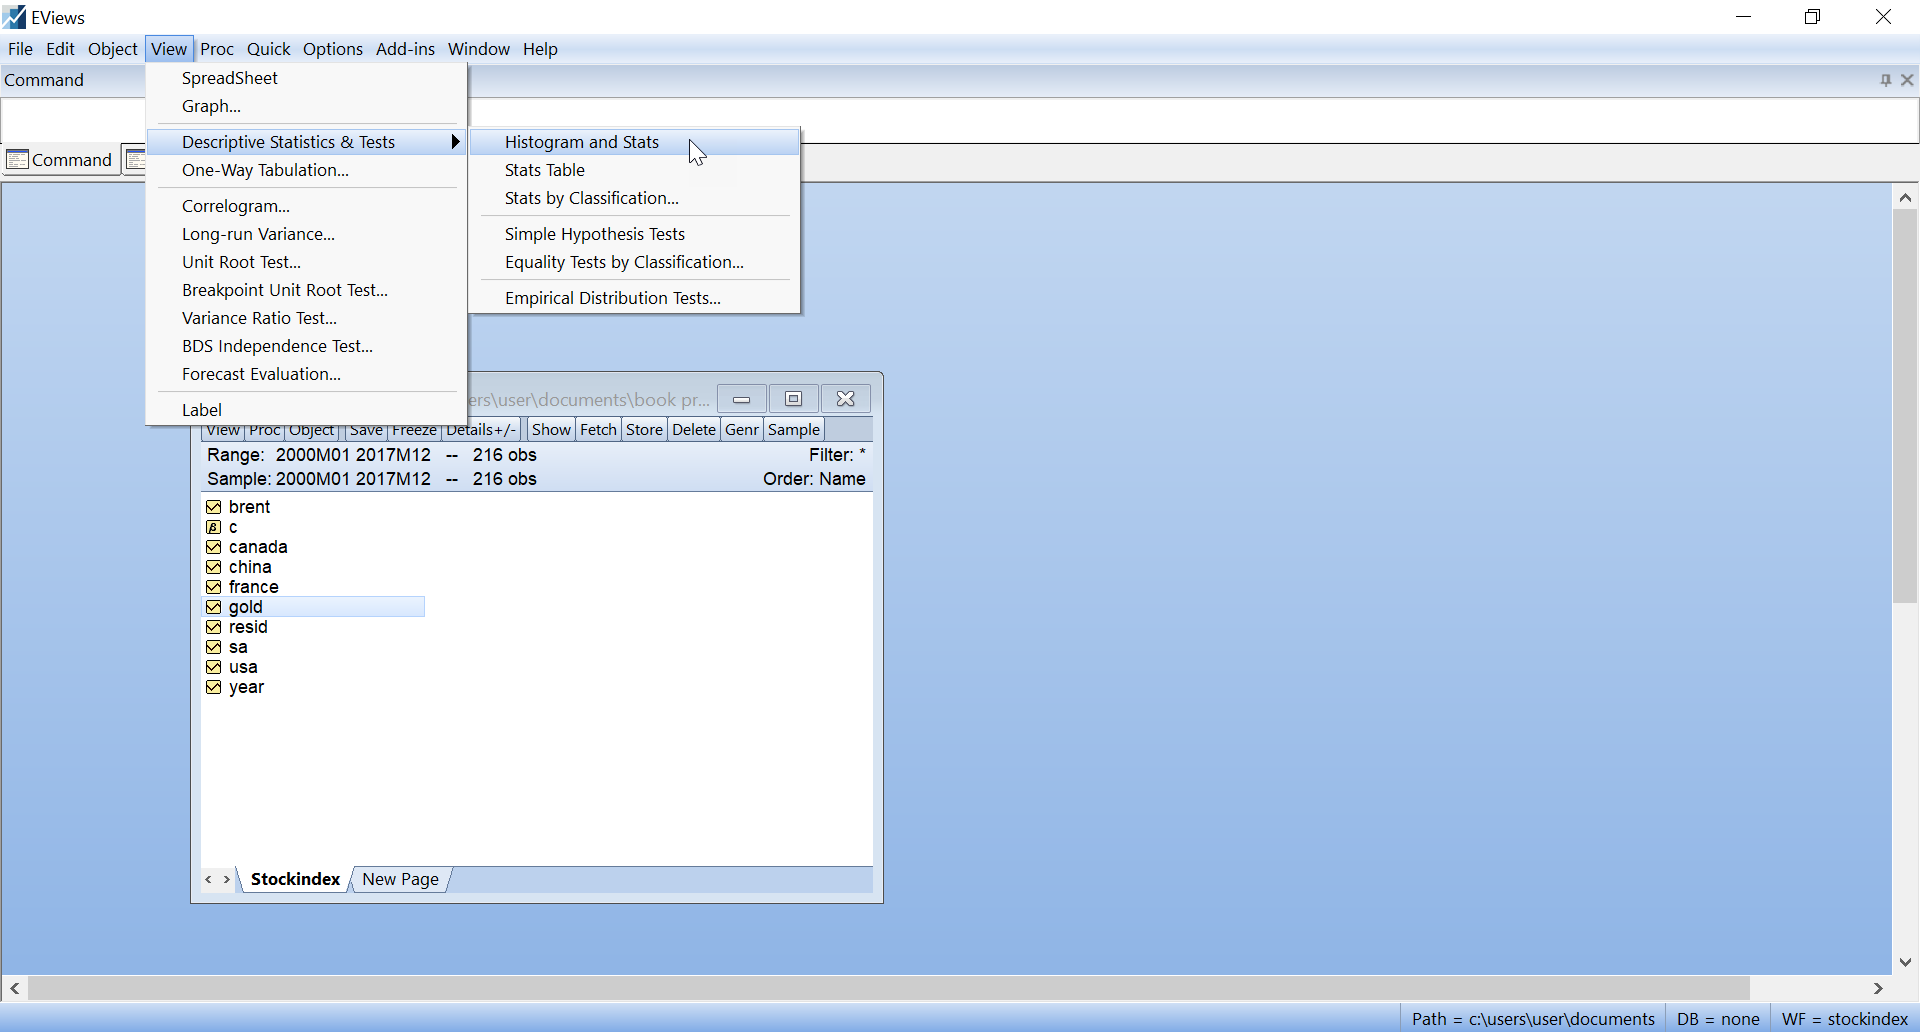
\includegraphics{images/descriptive2-01.png}
\item
  The descriptive statistics is displayed below in the dialog box below.

  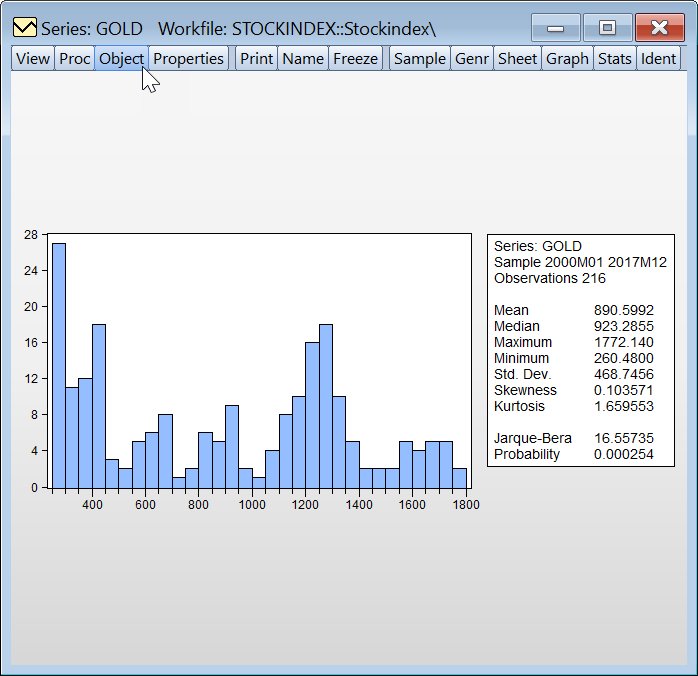
\includegraphics{images/descriptive3result.png}
\end{enumerate}

Click on

Alternatively, this step depends on the version of EViews you are using

\begin{enumerate}
\def\labelenumi{\arabic{enumi}.}
\tightlist
\item
  Choose the statistics you want to compute, such as mean, median,
  standard deviation, variance, skewness, kurtosis, etc.
\item
  Click the ``OK'' button to generate the descriptive statistics table.
\end{enumerate}

\hypertarget{step-4-descriptive-statistics-for-categorical-variables}{%
\subsubsection{\texorpdfstring{\textbf{Step 4: Descriptive Statistics
for Categorical
Variables}}{Step 4: Descriptive Statistics for Categorical Variables}}\label{step-4-descriptive-statistics-for-categorical-variables}}

\begin{enumerate}
\def\labelenumi{\arabic{enumi}.}
\tightlist
\item
  If you have categorical variables (e.g., a variable with categories
  like ``Yes'' or ``No''), you can create frequency tables to summarize
  them.
\item
  Go to ``View'' \textgreater{} ``Quick'' \textgreater{} ``Frequency.''
\item
  Select the categorical variable you want to analyze.
\item
  Click the ``OK'' button to generate a frequency table.
\end{enumerate}

\hypertarget{step-5-histograms-and-graphical-summaries}{%
\subsubsection{\texorpdfstring{\textbf{Step 5: Histograms and Graphical
Summaries}}{Step 5: Histograms and Graphical Summaries}}\label{step-5-histograms-and-graphical-summaries}}

This step is for EViews 14

\begin{enumerate}
\def\labelenumi{\arabic{enumi}.}
\item
  To visualize the distribution of numeric variables, you can create
  histograms and other graphical summaries.
\item
  Go to ``Graph'' \textgreater{} ``Create'' \textgreater{}
  ``Histogram.''
\item
  Select the variable you want to create a histogram for and configure
  the settings as desired.
\end{enumerate}

Click ``OK'' to generate the histogram.

\textbf{Step 6: Summary Statistics for Time Series Data}

\begin{enumerate}
\def\labelenumi{\arabic{enumi}.}
\item
  If you're working with time series data, you can generate summary
  statistics such as autocorrelation and partial autocorrelation.
\item
  Go to ``Quick'' \textgreater{} sieries statistics \textgreater{}
  ``Auto/Partial Auto-Correlation.''
\item
  Select the time series variable you want to analyze.
\item
  Configure the lag values and options, then click ``OK'' to generate
  the statistics.
\end{enumerate}

\hypertarget{step-7-exporting-results}{%
\subsubsection{\texorpdfstring{\textbf{Step 7: Exporting
Results}}{Step 7: Exporting Results}}\label{step-7-exporting-results}}

\begin{enumerate}
\def\labelenumi{\arabic{enumi}.}
\item
  You can export your descriptive statistics or graphical summaries by
  going to ``File'' \textgreater{} ``Export'' and selecting your desired
  file format (e.g., Excel, text).
\item
  Save the file in your preferred location.
\end{enumerate}

These steps cover basic descriptive statistics in EViews. Depending on
your specific analysis requirements, you can explore more advanced
statistical tools and techniques available in EViews for a deeper
understanding of your data.

\hypertarget{visualizing-time-series-data-using-charts-and-graphs.}{%
\subsection{Visualizing time series data using charts and
graphs.}\label{visualizing-time-series-data-using-charts-and-graphs.}}

Visualizing time series data using charts and graphs is an essential
step in exploring and understanding the underlying patterns, trends, and
anomalies in your data. In EViews, you can create various types of time
series charts and graphs to visually represent your data. Here's a
step-by-step guide on how to visualize time series data using charts and
graphs in EViews:

\hypertarget{step-1-load-your-time-series-data}{%
\subsubsection{\texorpdfstring{\textbf{Step 1: Load Your Time Series
Data}}{Step 1: Load Your Time Series Data}}\label{step-1-load-your-time-series-data}}

\begin{enumerate}
\def\labelenumi{\arabic{enumi}.}
\item
  Open EViews.
\item
  Load your time series data by going to ``File'' \textgreater{}
  ``Open'' and selecting your EViews workfile containing the time series
  data.
\end{enumerate}

\hypertarget{step-2-create-a-line-chart}{%
\subsubsection{\texorpdfstring{\textbf{Step 2: Create a Line
Chart}}{Step 2: Create a Line Chart}}\label{step-2-create-a-line-chart}}

A line chart is a fundamental visualization for time series data. It
displays data points connected by lines, making it easy to observe
trends and fluctuations over time.

\begin{enumerate}
\def\labelenumi{\arabic{enumi}.}
\item
  Click on ``Quick'' in the main menu.
\item
  Select ``Graph'' \textgreater{} ``Line Graph.''
\end{enumerate}

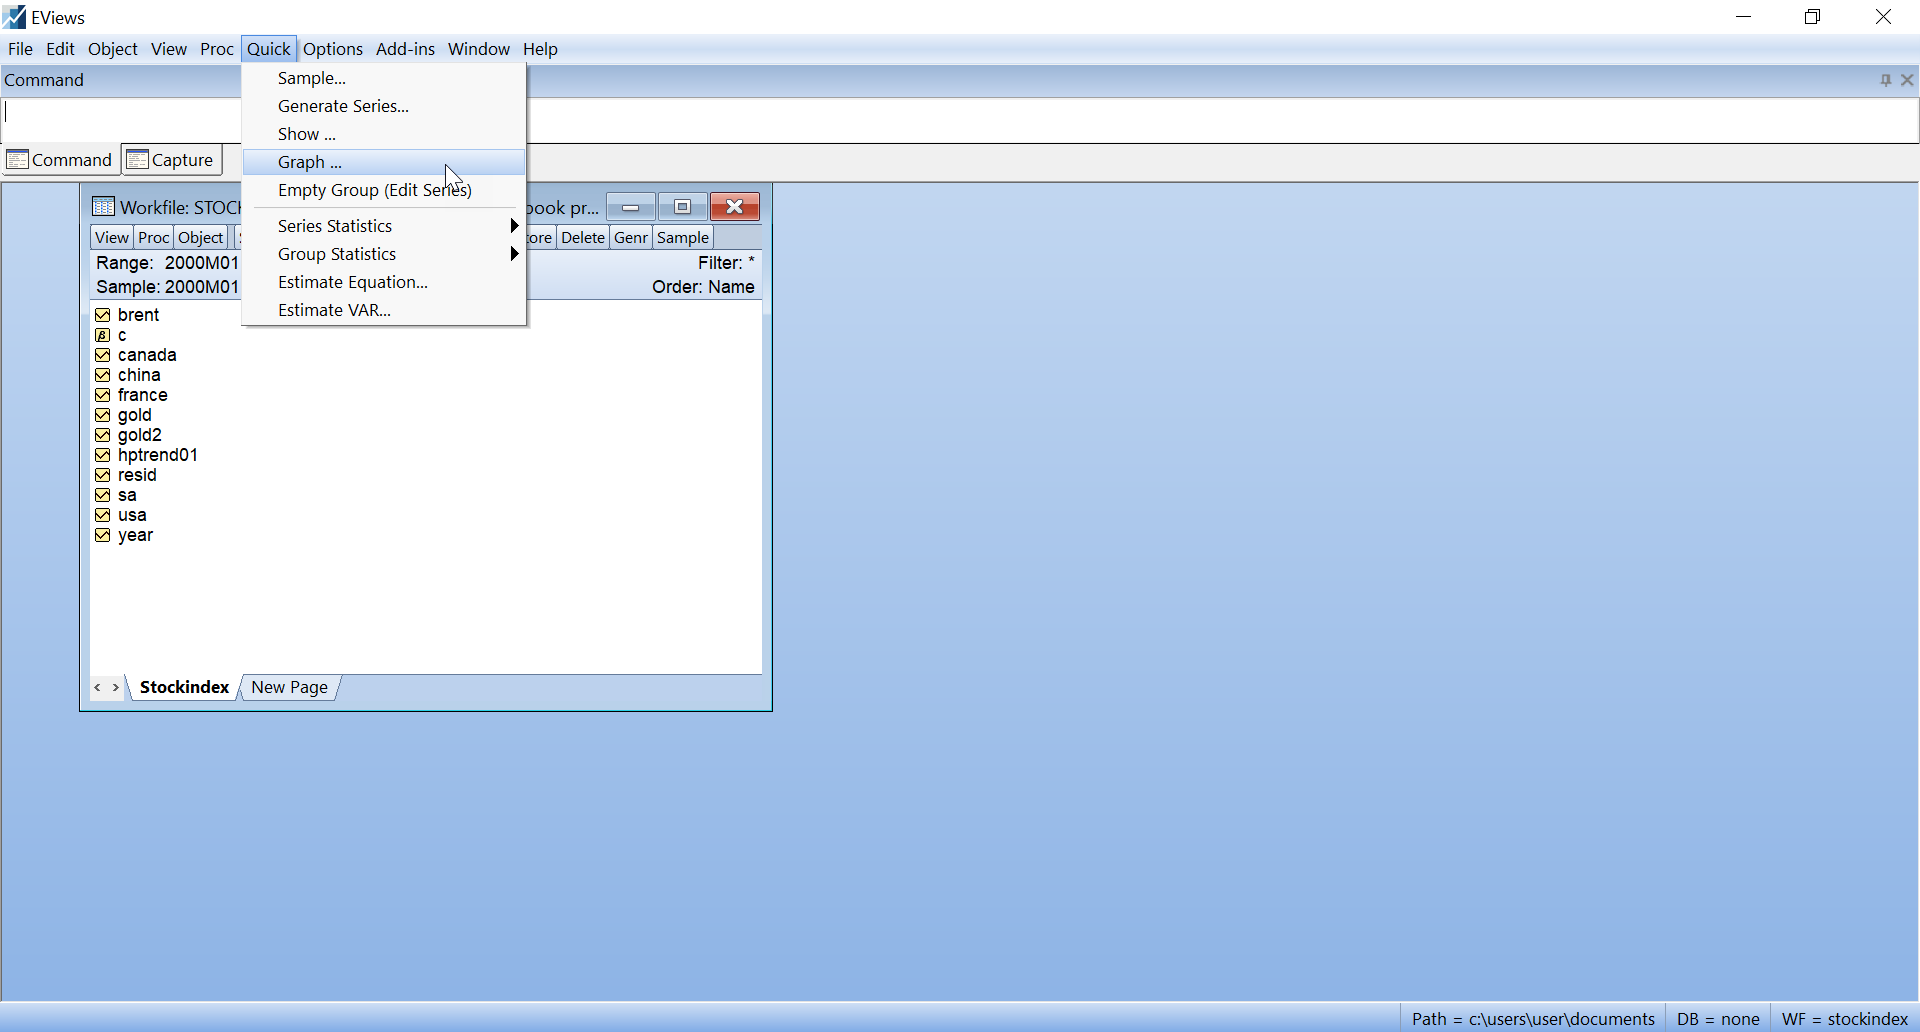
\includegraphics{images/graphimport1.png}

\begin{enumerate}
\def\labelenumi{\arabic{enumi}.}
\item
  In the ``Line Graph'' dialog box:

  \begin{itemize}
  \tightlist
  \item
    Choose the time series variable you want to visualize as the
    ``Series.''
  \end{itemize}

  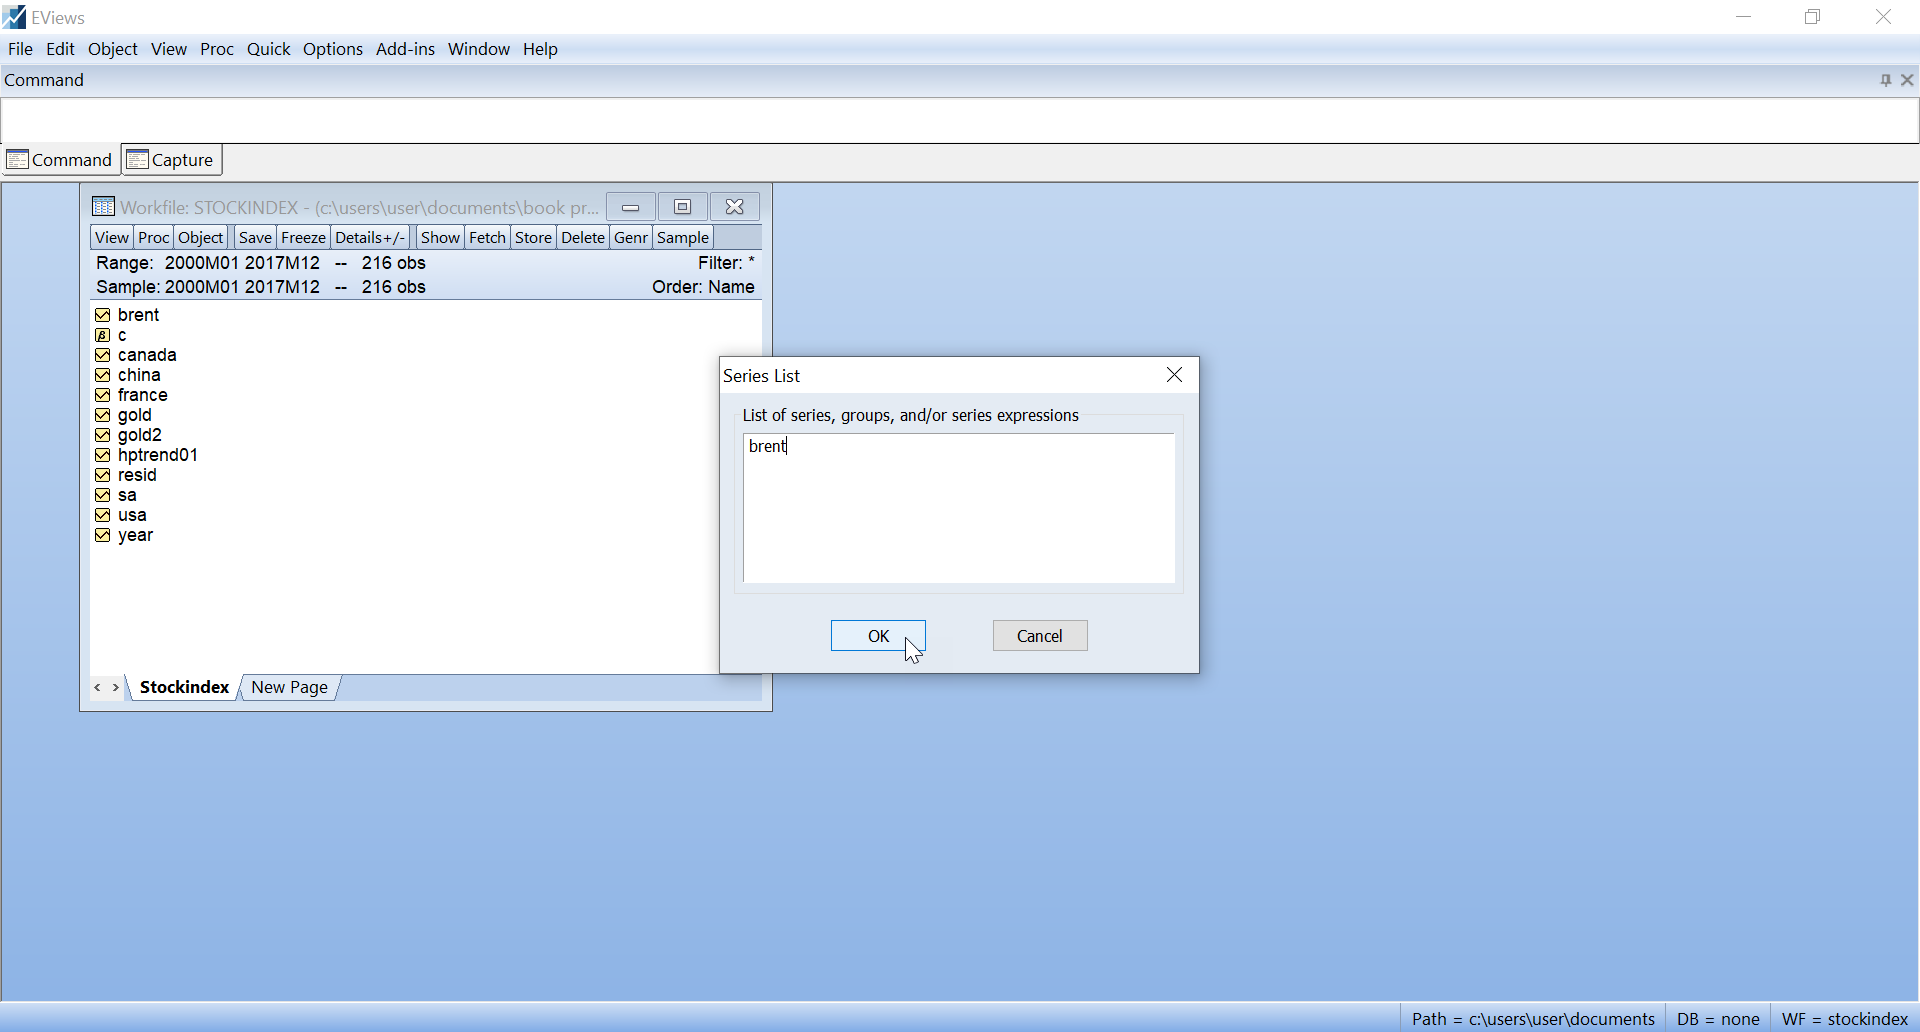
\includegraphics{images/graphimport3.png}

  \begin{itemize}
  \item
    Specify the X-axis variable (usually, the time variable).
  \item
    Customize chart settings like title, axis labels, and appearance.

    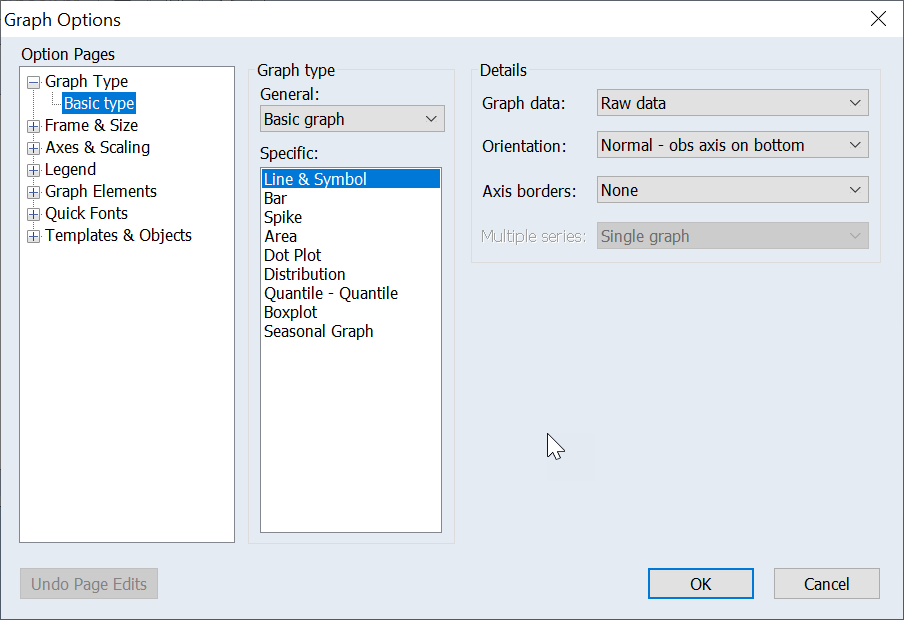
\includegraphics{images/graphimport4.png}
  \item
    Click ``OK'' to generate the line chart.

    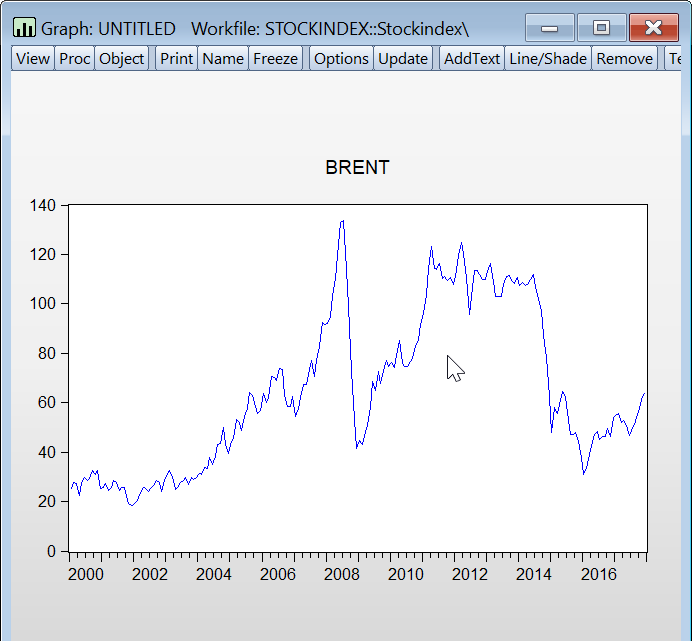
\includegraphics{images/graphimport5.png}
  \end{itemize}
\end{enumerate}

\hypertarget{step-3-create-a-scatter-plot}{%
\subsubsection{\texorpdfstring{\textbf{Step 3: Create a Scatter
Plot}}{Step 3: Create a Scatter Plot}}\label{step-3-create-a-scatter-plot}}

A scatter plot is useful for visualizing the relationship between two
time series variables. You can use it to assess correlations and
potential patterns.

\begin{enumerate}
\def\labelenumi{\arabic{enumi}.}
\item
  Click on ``Quick'' in the main menu.
\item
  Select ``Graph'' \textgreater{} type any two variables you intend to
  plot. Note that the variable name must be exact with the name on the
  workfile.
\item
  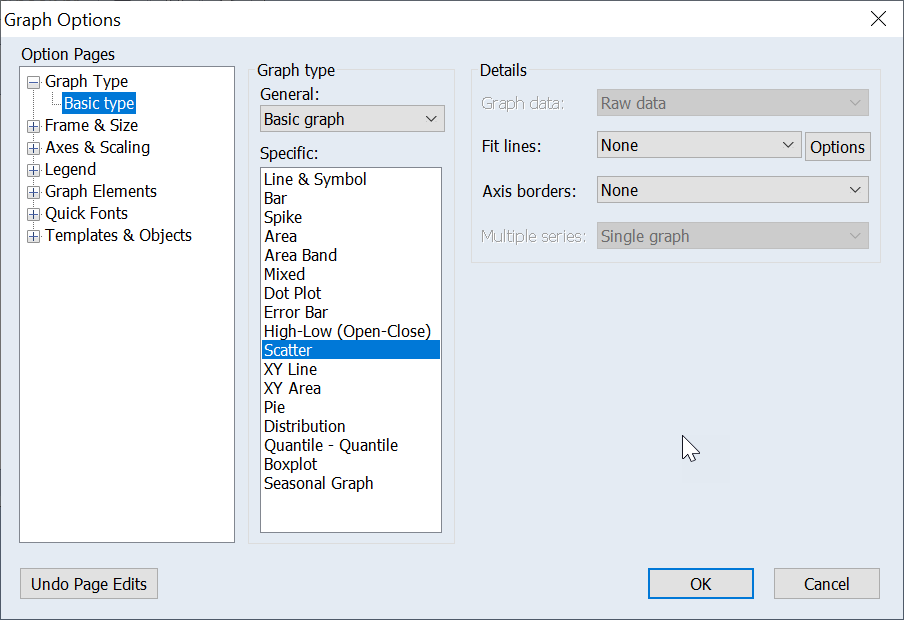
\includegraphics{images/scatterplot2.png}
\end{enumerate}

\begin{enumerate}
\def\labelenumi{\arabic{enumi}.}
\item
  In the ``Scatter Plot'' dialog box:

  \begin{itemize}
  \item
    Choose the two time series variables for the X-axis and Y-axis.
  \item
    Customize chart settings like title, axis labels, and appearance.
  \end{itemize}
\item
  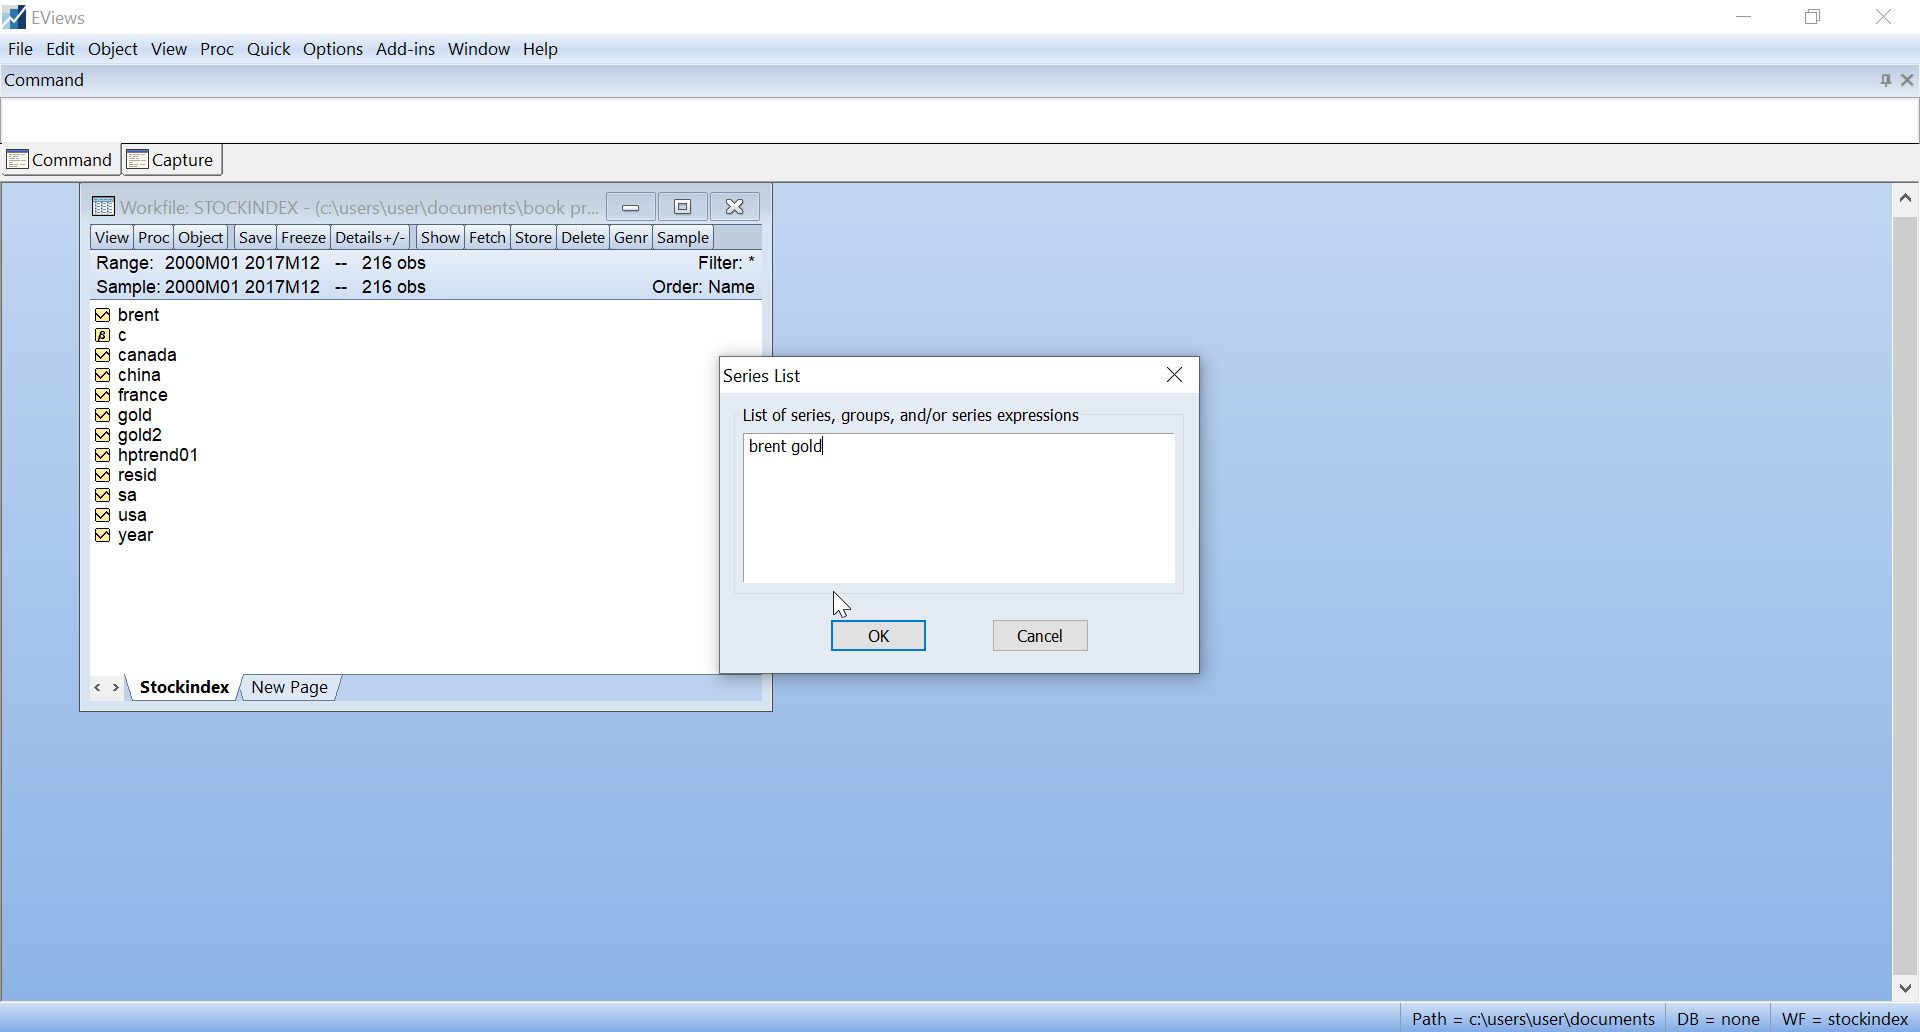
\includegraphics{images/correlation1.png}

  \begin{itemize}
  \item
    Click ``OK'' to generate the scatter plot.

    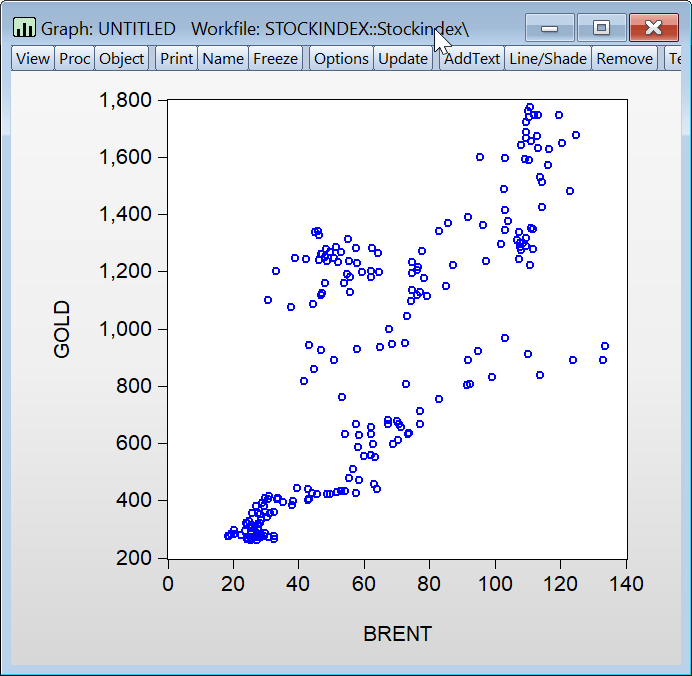
\includegraphics{images/scatterplot3.png}
  \end{itemize}

  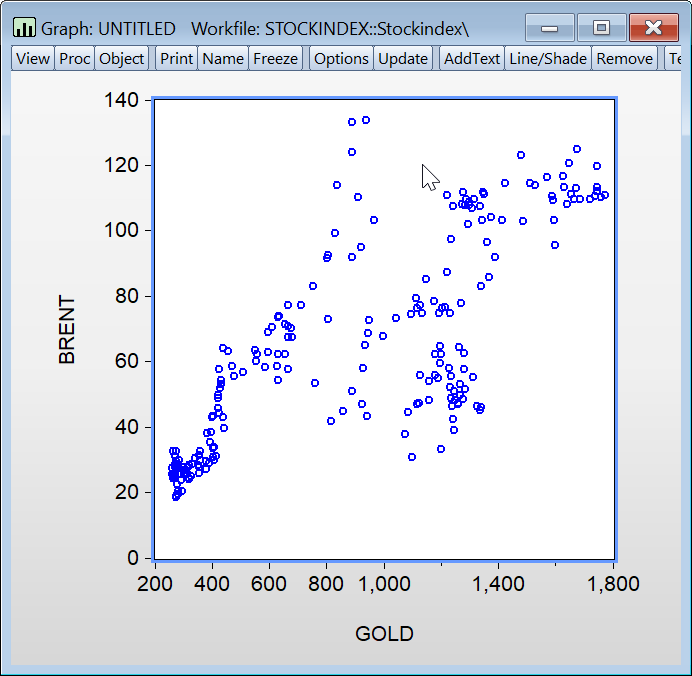
\includegraphics{images/scatterplot.png}
\end{enumerate}

\hypertarget{step-4-create-other-types-of-graphs}{%
\subsubsection{\texorpdfstring{\textbf{Step 4: Create Other Types of
Graphs}}{Step 4: Create Other Types of Graphs}}\label{step-4-create-other-types-of-graphs}}

EViews offers additional types of graphs, such as bar charts, box plots,
and more. You can explore these options to visualize your time series
data from different perspectives.

\begin{itemize}
\item
  \textbf{Load or Enter Data}:

  Open EViews and load your data into a workfile.
\item
  \textbf{Select Your Series}:

  \begin{itemize}
  \item
    Identify the time series data you want to plot. Ensure it's
    available in your workfile.

    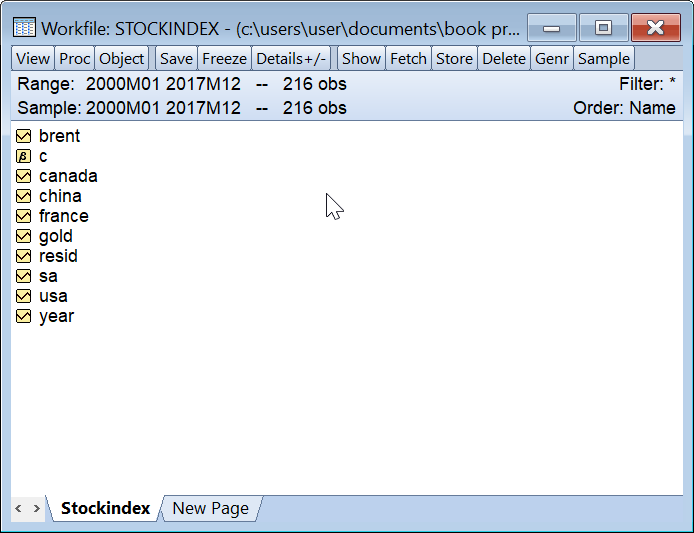
\includegraphics[width=5.625in,height=\textheight]{images/saveworkfile3-01.png}
  \end{itemize}
\item
  \textbf{Create a Line Graph}:

  \begin{itemize}
  \item
    Click on ``Quick'' in the top menu and type the variable name you
    want to plot on a graph in the `series list' dialog box.

    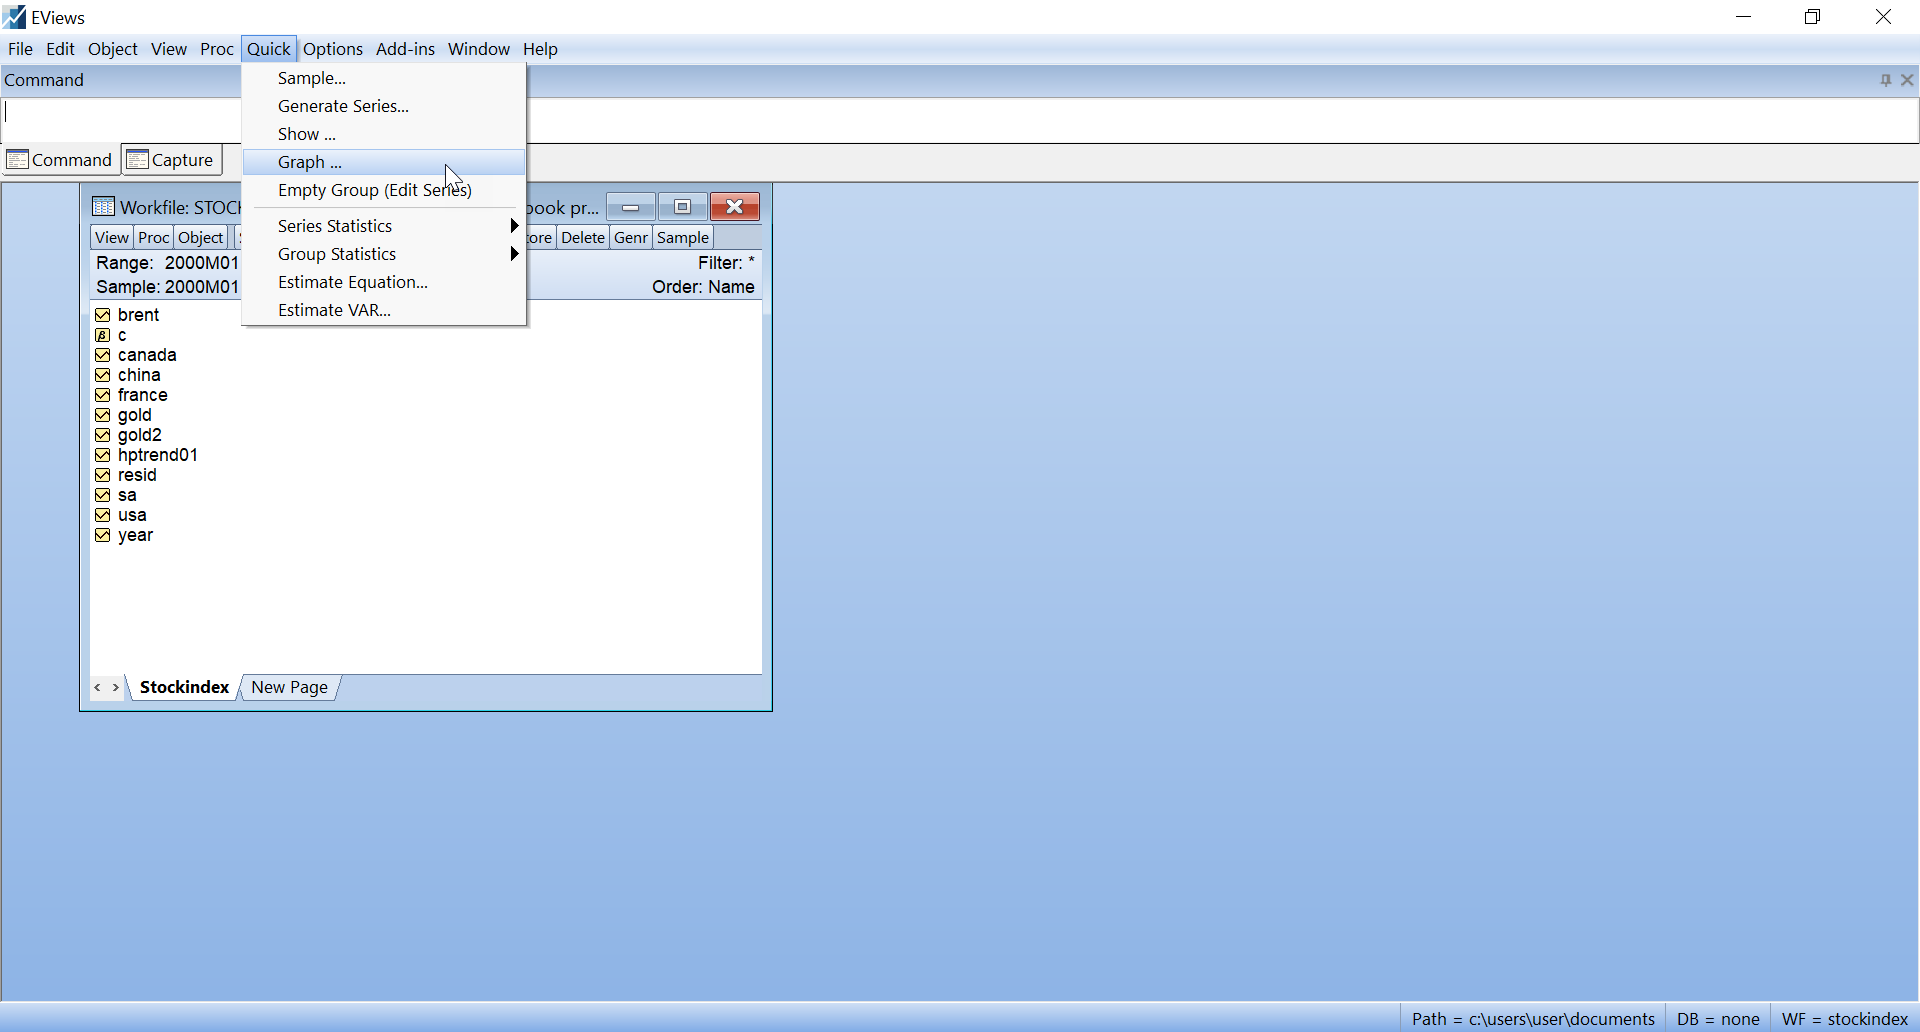
\includegraphics{images/graphimport1-01.png}
  \item
    In the graph dialog, under ``Graph type,'' select ``Line'' for a
    line graph.
  \end{itemize}
\item
  \textbf{Choose Series}:

  \begin{itemize}
  \item
    In the ``Series List'' dialog box, type the data series you want to
    plot. You can also select additional series for multiple lines on
    the graph. In this case we select multiple variables: brent canada
    china france gold sa usa
  \item
    Click ok

    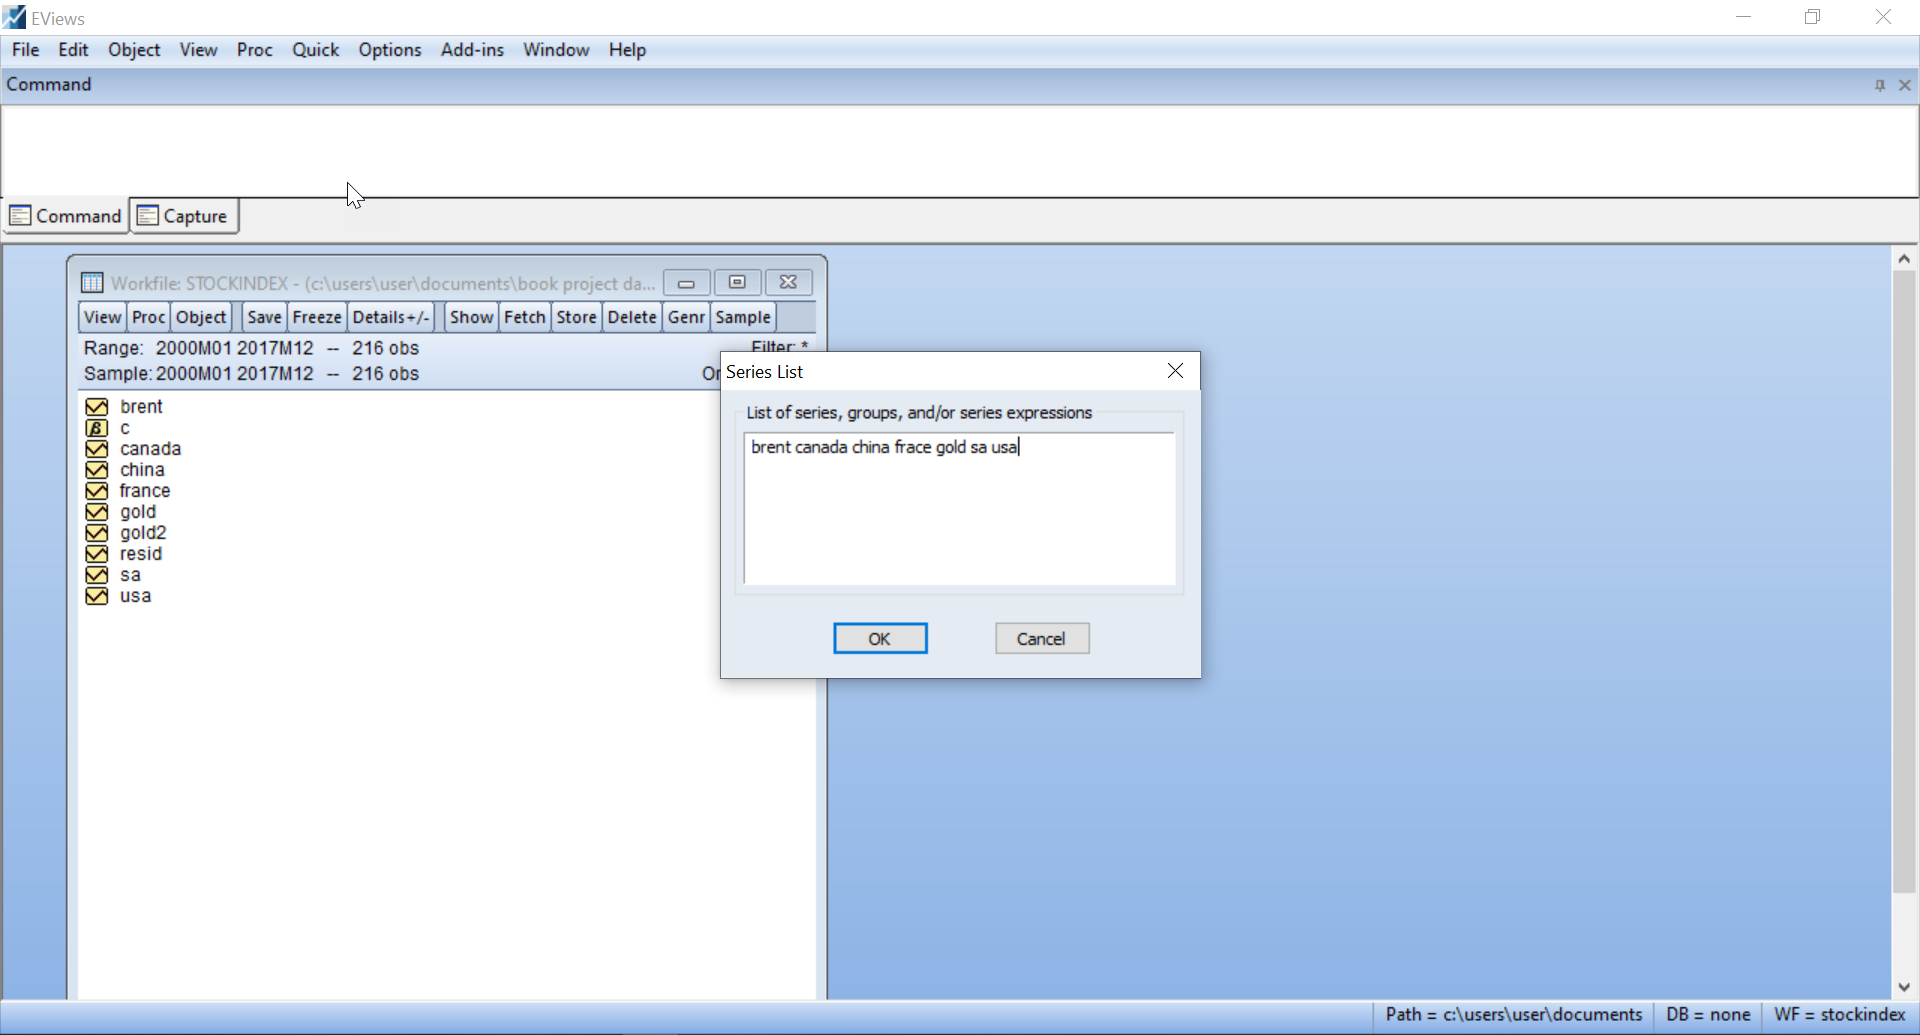
\includegraphics{images/linegraphimport.png}
  \item
    from the graph option dialog box, select line \& symbols in the
    specific section as shown below

    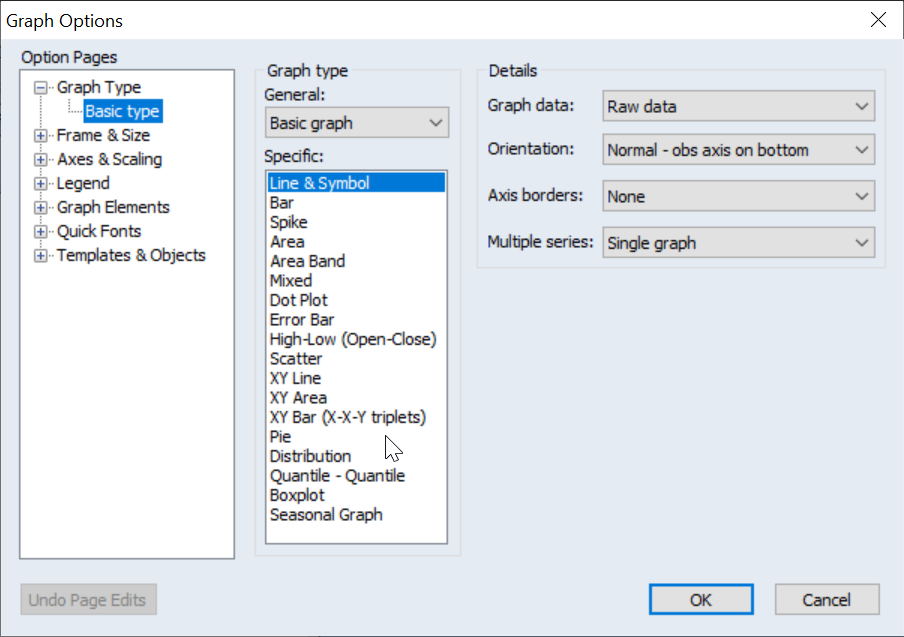
\includegraphics{images/linegraphimport2.png}

    \begin{itemize}
    \tightlist
    \item
      click ok to multiple timeseries plot is displayed.
    \end{itemize}
  \item
  \item
    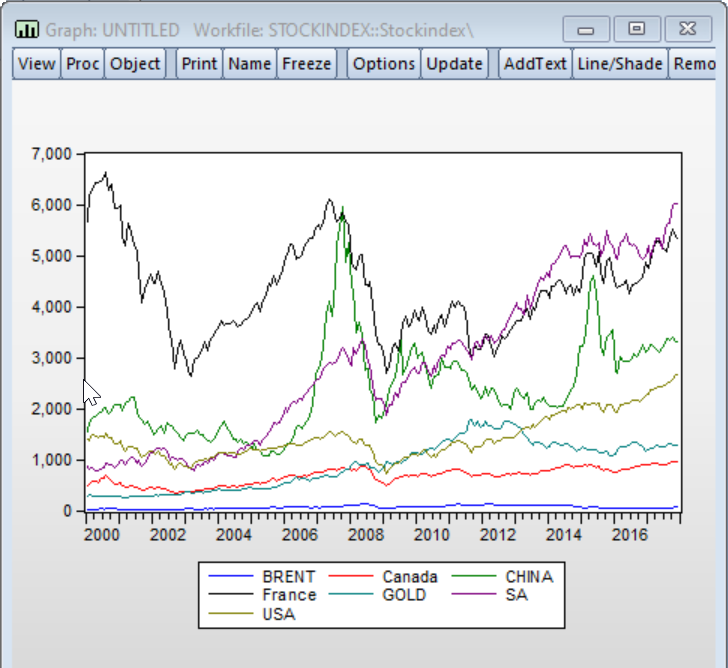
\includegraphics{images/linegraphimport3multiple.png}
  \item
    repeat the process and this time select multiple
  \item
    note the in the graph options dialog box below, you can select
    different kinds of graphs and plots including Bar, spike, area, area
    bank, mixed, dotplot eror bar among many others
  \end{itemize}
\end{itemize}

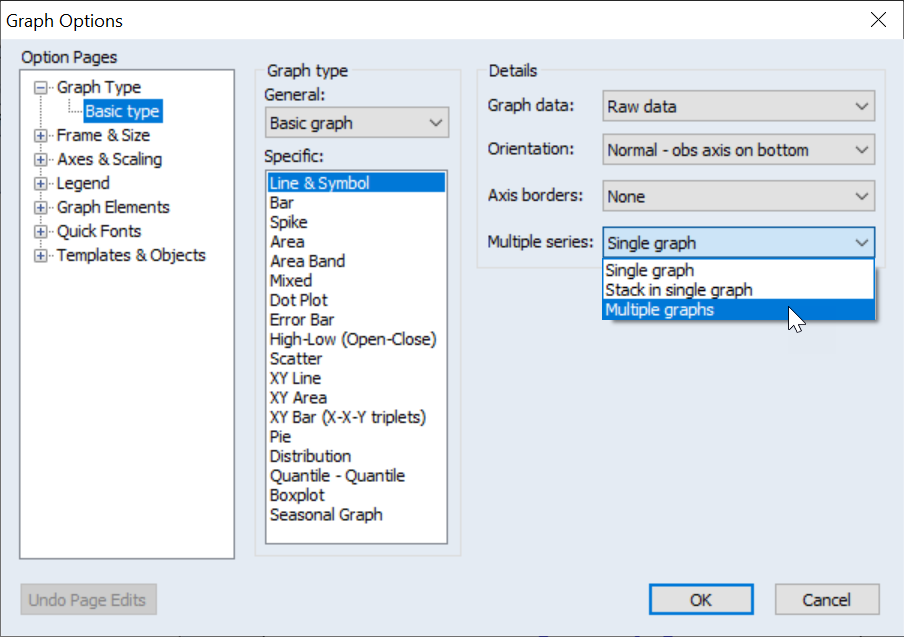
\includegraphics{images/linegraphimportmultiple2.png}

\begin{itemize}
\item
  click on multipl graphs
\item
  click ok to display the multiple graphs
\end{itemize}

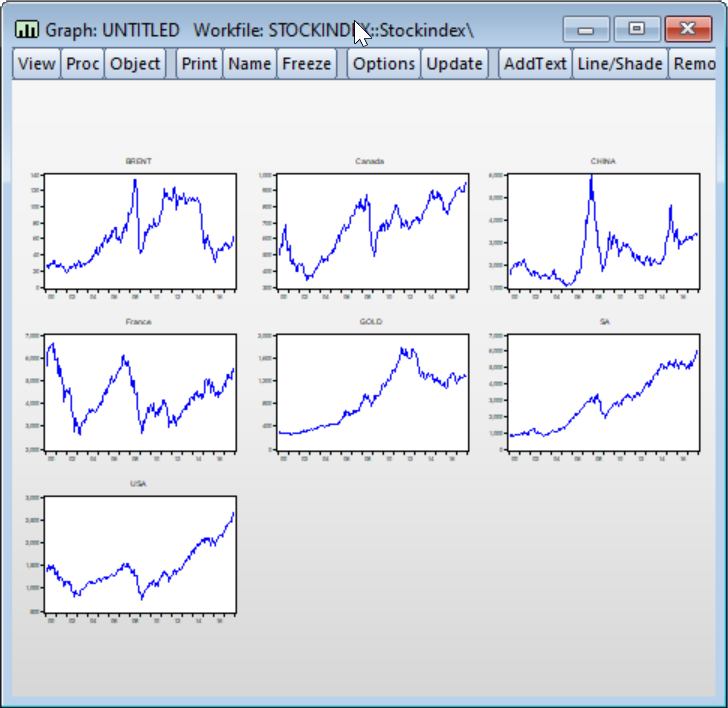
\includegraphics{images/linegraphmultiple3.png}

you can copy and paste any of the graphs into your Microsoft word file

other plots you can make from the same process and steps by choosing the
option of your choices:

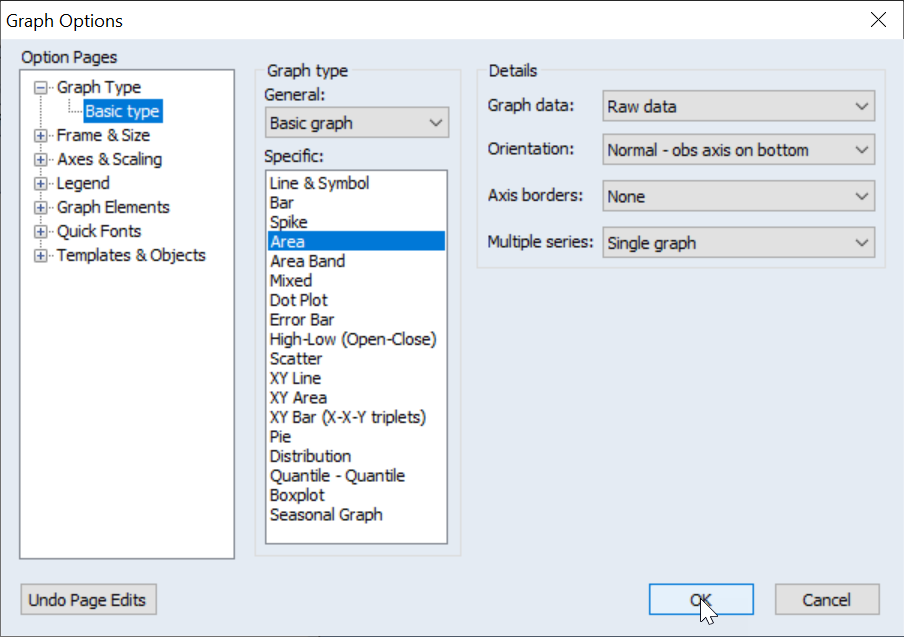
\includegraphics{images/areagraph-01.png}

\begin{figure}

{\centering 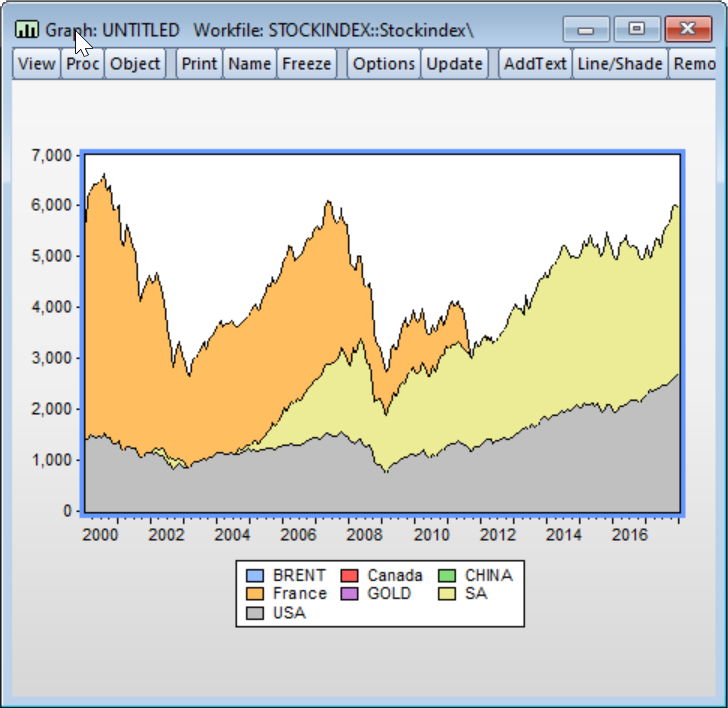
\includegraphics{images/2023-10-14_23-58-22.png}

}

\caption{Area Plot}

\end{figure}

\begin{figure}

{\centering 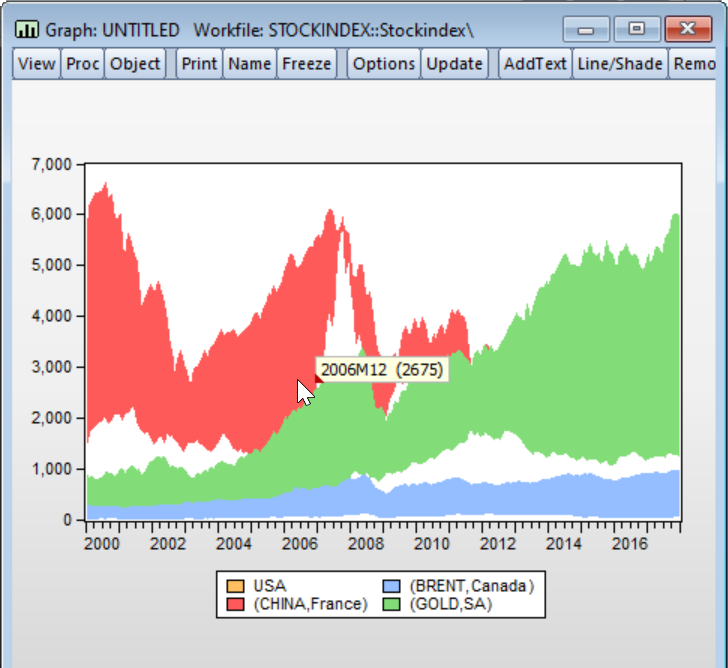
\includegraphics{images/areaplot2.png}

}

\caption{Area Band Plot}

\end{figure}

\begin{figure}

{\centering 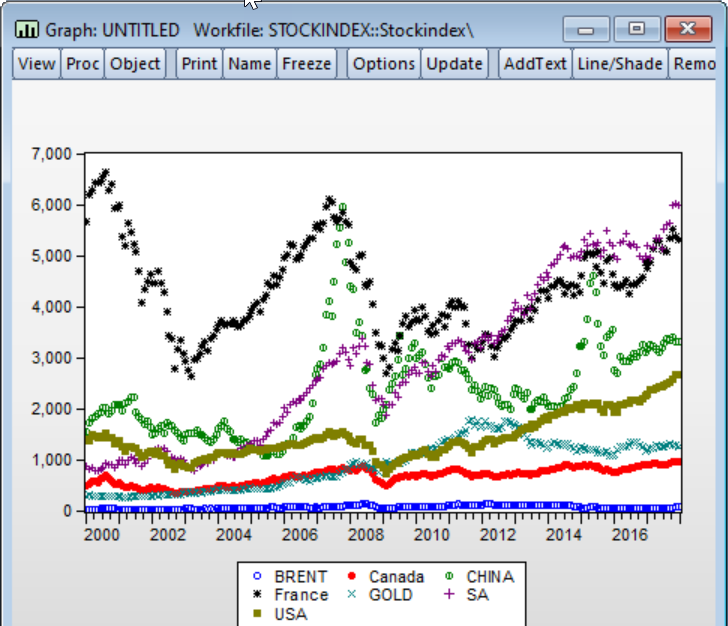
\includegraphics{images/dotplot.png}

}

\caption{Dot Plot}

\end{figure}



\end{document}
